\documentclass[11pt]{beamer}

%------------------------------------------------
%   PAQUETES
%------------------------------------------------
\usepackage[utf8]{inputenc}
\usepackage[T1]{fontenc}
\usepackage[spanish]{babel}
\usepackage{amsmath, amsfonts, amssymb}
\usepackage{graphicx}
\usepackage{enumerate}
\usepackage{mathrsfs}
\usepackage{color}
\usepackage{bm}

%------------------------------------------------
%   TEMA
%------------------------------------------------
\usetheme{Madrid}
\usecolortheme{default}

%------------------------------------------------
%   DATOS
%------------------------------------------------
\title{Generalización de las soluciones para la ecuación de onda con distintas
	condiciones acústicas en la frontera}

\author[Juan Luis Aguayo Lazcano]{Juan Luis Aguayo Lazcano\\
	\small Profesor Responsable: Dr.\ Andrés Ávila Barrera}

\date{Temuco, 22 de Abril de 2014}

%------------------------------------------------
%   DOCUMENTO
%------------------------------------------------
\begin{document}
	
	%------------------------------------------------
	\begin{frame}
		\begin{figure}[l]
			\begin{minipage}{1cm}
				\begin{center}
					
\includegraphics[scale=0.1]{logo.png}
				\end{center}
			\end{minipage}
			\hfill
			\begin{minipage}{0.85\textwidth}
				{\scriptsize Universidad de La Frontera\\
					Vicerrectoría de Investigación y Postgrado\\
					Doctorado en Ciencias Mención Matemática}
			\end{minipage}
		\end{figure}
		
		\vspace{-2mm}
		\hrule height 0.5pt width 4.25in
		\vspace{1mm}
		
		\titlepage
	\end{frame}
	
	%------------------------------------------------
	\section{Outline}
	\begin{frame}{Contenido}
		\begin{enumerate}
			\item Motivación 
			\item Introducción a la Teoría de Semigrupos
			\item Estabilidad Exponencial
			\item Estabilidad Polinomial
			\item Problema Acústico
		\end{enumerate}
	\end{frame}
	
	%------------------------------------------------
	\section{Motivación}
	
	\begin{frame}{El modelo físico y la ecuación de onda}
		\begin{center}
			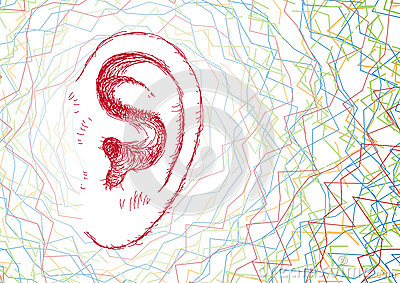
\includegraphics[width=220pt]{fig1.png}
		\end{center}
	\end{frame}
	
	\begin{frame}
		Dado un gas contenido en una caja...
	\end{frame}
	
	\begin{frame}
		Según la segunda Ley de Newton 
		\begin{equation}\label{eq1}
			\frac{\Delta F}{\Delta V}=-\nabla p=\rho\frac{D{\bf q}}{Dt}
		\end{equation}
		
		donde ${\bf q}$ representa la velocidad vectorial media, $\rho$ la densidad 
		instantánea, etc.
		
		\[
		\frac{D{\bf q}}{Dt}=\frac{\partial{\bf q}}{\partial t}+{\bf q}\cdot\nabla{\bf q}
		\]
	\end{frame}
	
	\begin{frame}
		Si ${\bf q}$ es pequeña entonces $D{\bf q}/Dt \approx \partial{\bf q}/\partial t$:
		
		\begin{equation}
			-\nabla p=\rho_0\frac{\partial{\bf q}}{\partial t}
		\end{equation}
		
		Ley de Charles–Boyle:
		
		\[
		PV^\gamma = C
		\]
	\end{frame}
	
	\begin{frame}
		Diferenciando:
		
		\[
		\frac{1}{P}\frac{dP}{dt} = -\gamma \frac{1}{V}\frac{dV}{dt}
		\]
		
		Sean:
		
		\[
		P=P_0+p,\qquad V=V_0+\tau
		\]
	\end{frame}
	
	\begin{frame}
		Dado que $p\ll P_0$ y $\tau \ll V_0$:
		
		\[
		\frac{p}{P_0} = -\gamma \frac{\tau}{V_0}
		\]
		
		Derivando:
		
		\[
		\frac{1}{P_0}\frac{\partial p}{\partial t}
		= -\frac{\gamma}{V_0}\frac{\partial\tau}{\partial t}
		\]
	\end{frame}
	
	\begin{frame}
		La variación de volumen es
		
		\[
		\tau = V_0 \, \text{div}\,\xi
		\]
		
		y
		
		\[
		\frac{\partial \tau}{\partial t} = V_0\,\text{div}\,{\bf q}
		\]
		
		Combinando ecuaciones:
		
		\[
		\frac{\partial p}{\partial t} = -\gamma P_0 \, \text{div}\,{\bf q}
		\]
	\end{frame}
	
	\begin{frame}
		Diferenciando y comparando con
		
		\[
		-\nabla^2 p = \rho_0\ \text{div}\left(\frac{\partial{\bf q}}{\partial t}\right)
		\]
		
		se obtiene:
		
		\[
		\nabla^2 p = \frac{\rho_0}{\gamma P_0}\frac{\partial^2 p}{\partial t^2}
		\]
		
		Sea $c^2=\gamma P_0/\rho_0$:
		
		\[
		\Delta p = \frac{1}{c^2} p_{tt}
		\]
	\end{frame}
	
	%------------------------------------------------
	% Tipos de ondas
	%------------------------------------------------
	
	\begin{frame}{Tipos de ondas}
		\begin{center}
			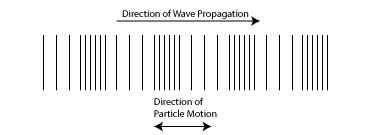
\includegraphics[width=250pt]{fig3.png}
		\end{center}
	\end{frame}
	
	\begin{frame}
		\begin{center}
			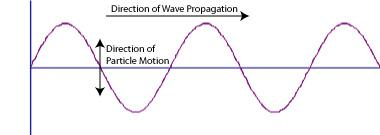
\includegraphics[width=200pt]{fig4.png}
			
			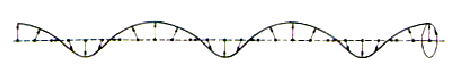
\includegraphics[width=200pt]{fig5.png}
		\end{center}
	\end{frame}
	
	\begin{frame}
		\begin{center}
			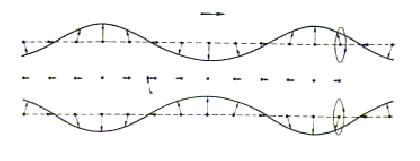
\includegraphics[width=200pt]{fig6.png}
			
			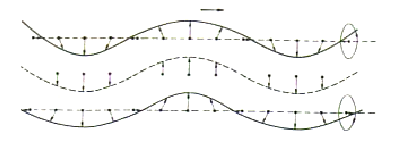
\includegraphics[width=200pt]{fig7.png}
		\end{center}
	\end{frame}
	
	%------------------------------------------------
	\begin{frame}
		\centerline{\huge Ejemplos de la ecuación de onda}
	\end{frame}
	
	\begin{frame}
		Problema 1: cuerda vibrante.
		\[
		u_{tt}=c^2 u_{xx},\qquad 0<x<L
		\]
	\end{frame}
	
	\begin{frame}
		Problema 2: viga vibratoria.
		\[
		c^2 u_{xxxx}+u_{tt}=0
		\]
	\end{frame}
	
	\begin{frame}
		Problema 3: membrana circular.
		\[
		u_{tt}=c^2\left(u_{rr}+\frac{1}{r}u_r\right)
		\]
	\end{frame}
	
	%------------------------------------------------
	\begin{frame}
	\end{frame}
	%------------------------------------------------
	
	\section{Teoría de Semigrupos}
	
	\begin{frame}
		\centerline{\huge Introducción a los Semigrupos}
	\end{frame}
	
	\begin{frame}
		Problema de valor inicial:
		
		\[
		u_{tt}-\alpha u_{xx}=0
		\]
		
		Reescritura como sistema de primer orden:
		
		\[
		U=\begin{pmatrix}u\\u_t\end{pmatrix}
		\]
	\end{frame}
	
	\begin{frame}
		Definición del problema abstracto:
		
		\[
		U_t = AU,\qquad U(0)=U_0
		\]
	\end{frame}
	
	\begin{frame}{Aspectos básicos}
		Exponencial:
		
		\[
		e^{tA}=\sum_{n=0}^\infty \frac{(tA)^n}{n!}
		\]
	\end{frame}
	
	\begin{frame}
		Definición de semigrupo:
		
		\begin{itemize}
			\item $T(0)=I$
			\item $T(t+s)=T(t)T(s)$
		\end{itemize}
	\end{frame}
	
	\begin{frame}
		Definición del generador infinitesimal:
		
		\[
		A x = \lim_{h\to 0} \frac{T(h)x - x}{h}
		\]
	\end{frame}
	
	\begin{frame}
		Si $T(t)$ es uniformemente continuo:
		
		\[
		\|T(t)\|\le e^{\omega t}
		\]
	\end{frame}
	
	%------------------------------------------------
\end{document}
